\section{Angle droit ou pas ? }

%\begin{multicols}{2}
	\begin{center}
		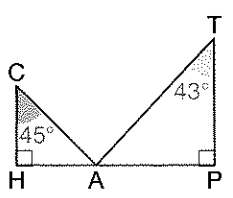
\includegraphics[scale=0.15]{img/fig}
	\end{center}
	
	Les points $H$, $A$  et $P$ sont alignés.
	
	\begin{questions}
		\question \`A partir des informations codées sur la figure et sans faire de mesure, dire si la triangle $CAT$ est rectangle en A. Justifier la réponse.
	\end{questions}
	\begin{solution}
		Calcul de la mesure de l'angle \monAngle{CAH} :
		
		Dans le triangle CAH, on a \monAngle{C} + \monAngle{A} + \monAngle{H} = 180\degree.
		
			\begin{eqnarray*}
				\widehat{A}  &=& 180 - (\widehat{C} + \widehat{H}) \\
				\widehat{A}  &=& 180 - (45 + 90) \\
				\widehat{A}  &=& 45
			\end{eqnarray*}
		L'angle \monAngle{CAH} mesure 45\degree.\\
		
		
		
		Calcul de la mesure de l'angle \monAngle{TAP} :
		
		Dans le triangle TAP, on a \monAngle{T} + \monAngle{A} + \monAngle{P} = 180\degree.
		
		\begin{eqnarray*}
			\widehat{A}  &=& 180 - (\widehat{T} + \widehat{P}) \\
			\widehat{A}  &=& 180 - (43 + 90) \\
			\widehat{A}  &=& 47
		\end{eqnarray*}
		L'angle \monAngle{TAP} mesure 47\degree.\\
		
		Calcul de la mesure de l'angle \monAngle{CAT} :
		Je sais que les points $H$, $A$ et $P$ sont alignés donc \monAngle{HAP} mesure 180\degree.
		
		On a donc :
		
		\begin{eqnarray*}
			\widehat{CAT}  &=& 180 - (\widehat{CAH} + \widehat{TAP}) \\
			\widehat{CAT}  &=& 180 - (45 + 47) \\
			\widehat{CAT}  &=& 88
		\end{eqnarray*}
	
		L'angle \monAngle{CAT} mesure 88\degree et non 90\degree, donc le triangle $CAT$ n'est pas rectangle en $A$.
	\end{solution}



	
%\end{multicols}